\documentclass[a4paper, 12pt]{book}
\usepackage{graphicx}
\usepackage[french]{babel}
\usepackage[utf8]{inputenc}
\usepackage[T1]{fontenc}
\usepackage{multirow}
\usepackage{listings}
\usepackage{float}
\usepackage{url}
\usepackage[french]{algorithm}
\usepackage{style/myalgorithm}
\usepackage{amsmath,amsfonts,amssymb}
\newcommand{\fBm}{\emph{fBm}~}
\newcommand{\etal}{\emph{et al.}~}
\newcommand{\glAd}{\emph{GL4D}~}
\newcommand{\apiopengl}{API OpenGL\textsuperscript{\textregistered}~}
\newcommand{\opengl}{OpenGL\textsuperscript{\textregistered}~}
\newcommand{\opengles}{OpenGL\textsuperscript{\textregistered}ES~}
\newcommand{\clang}{langage \texttt{C}}
\newcommand{\codesource}{\textsc{Code source}~}
\floatstyle{ruled}
\newfloat{programslist}{htbp}{locs}
\newcommand{\listofprograms}{\listof{programslist}{Liste des codes source}}
\newcounter{program}[subsection]
\renewcommand{\theprogram}{\arabic{chapter}.\arabic{program}}

\newenvironment{program}[1]{
  \if\relax\detokenize{#1}\relax
  \gdef\mycaption{\relax}
  \else
  \gdef\mycaption{#1}
  \fi
  \refstepcounter{program}
  \addcontentsline{locs}{section}{#1}
  \footnotesize
}{
  \begin{description}
    \item[\codesource \theprogram]--~\mycaption
  \end{description}
}

\begin{document}
\begin{titlepage}
  \begin{center}
    \begin{tabular*}{\textwidth}{l@{\extracolsep{\fill}}r}
      
\includegraphics[height=1.5cm]{images/m2ise.png}
    \end{tabular*}
    \small 
    \rule{\textwidth}{.5pt}~\\
    \large 
    \textsc{Université Paris 8 - Vincennes à Saint-Denis}\vspace{0.5cm}\\
    \textbf{Master Informatique des Systèmes Embarqués}\vspace{3.0cm}\\
    \Large
    \textbf{Memoire de projet tuteuré}\vspace{1.5cm}\\
    \large
    \textbf{Fakhri \textsc{YAHIAOUI} - Roman \textsc{BOURSIER}}\vspace{1.5cm}\\
    Date de soutenance : le 09/06/2020\vspace{1.75cm}\\
  \end{center}\vspace{1.5cm}~\\
  \begin{tabular}{ll}
    \hspace{-0.45cm}Tuteur -- Université~:~&~Farès \textsc{BELHADJ}\\
  \end{tabular}
\end{titlepage}
\frontmatter
\chapter*{Résumé}
\markboth{\sc Résumé}{}
\addcontentsline{toc}{chapter}{Résumé} 

A faire en dernier ...


\chapter*{Remerciements}
\markboth{\sc Remerciements}{}
\addcontentsline{toc}{chapter}{Remerciements} 

Idem ...

%% Table des matières
\tableofcontents

\mainmatter
\chapter*{Introduction}
\markboth{\sc Introduction}{}
\addcontentsline{toc}{chapter}{Introduction}

\section{Contexte}
Dans le cadre de notre projet de fin d'étude, nous souhaitons utiliser des modèles d’apprentissage automatique (ex. Deep Learning) afin de produire un moteur de rendu capable d’adopter une stylisation « type » telle que la peinture chinoise. Dans un premier temps, il s’agira de proposer un modèle d’abstraction des peintures sélectionnées comme base d’apprentissage et d’utiliser le couple « peinture originale » / « abstraction » pour l’entraînement. Par la suite, un moteur de rendu d’abstractions sera connecté au réseau profond qui produira une peinture sur la base de l’abstraction.

Le modèle généré devra d'une part adopter la stylisation retenue mais aussi interpréter l'abstraction d'origine.


\chapter{Etat de l'art}
Nous présenterons dans ce chapitre les différents travaux en lien avec notre sujet. Nous traiterons des réseaux de neuronnes et plus particulièrement de l'architecture GAN. 

Nous évoquerons, de manière plus succincte, des récherches liées à notre sujet mais n'utilisant pas l'intelligence artificiel afin de pouvoir identifier les avantages et inconvénients des deux mondes. 


\section{Généralité sur les GANs}
Les réseaux adverses génératifs (en anglais generative adversarial networks ou GANs) sont une classe d'algorithmes d'apprentissage non-supervisé. Ces algorithmes ont été introduits par Goodfellow et al. 2014. Ils permettent de générer des images avec un fort degré de réalisme[1].

--- todo : plus de détails sur le fonctionnement des GANs

Il existe aujourd'hui une très grande variété de travaux de recherches implémentants les Gans (DCGAN, CGAN, Bayesian GAN, GYCLE GAN ...). Nous n'avons pas pu tous les étudier mais nous avons cependant orienté nos recherches sur les travaux autour du concept assez large du "transfert d'image ou de stylisation".




\section{Pix2Pix}

\section{GauGan}


\section{Le transfert de style neuronal}

Cette technique fut décrite par Leon A. Gatys dans son article "A Neural Algorithm of Artistic Style".~\cite{DBLP:journals/corr/GatysEB15a}

Celle-ci utilise trois images, la première est l'image d'entrée (bruit), la seconde représente le style de référence (comme une peinture par exemple), la dernière correspond à l'image que l'on souhaite transformer.

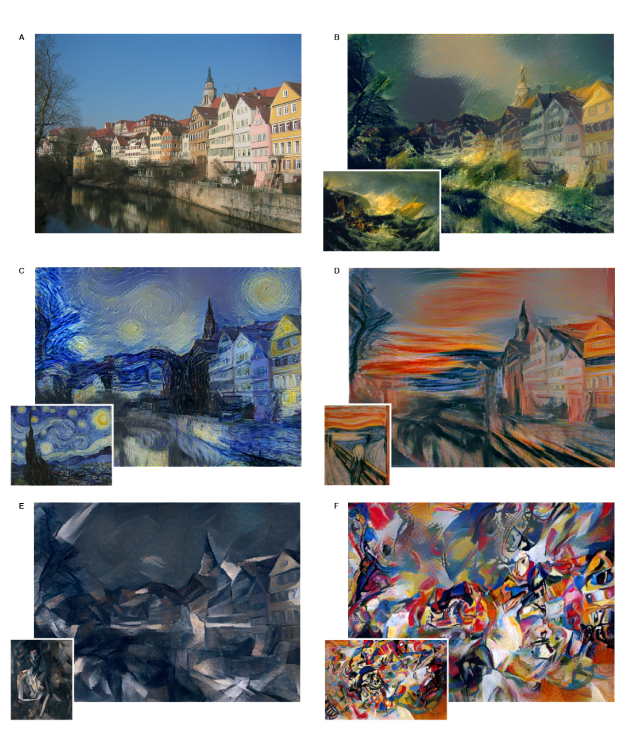
\includegraphics[width=0.7\linewidth]{images/neuronal-algorithm-artistic-style.png}

Le principe consiste à définir deux fonctions de distance. La première décrit comment le contenu de deux images sont différentes, et la seconde réprésente la différence de style. On obtient alors deux images, une pour le style souhaité, une pour le contenu.

L'objectif est de transformer l'image d'entrée en minimisant la distance avec l'image de contenu et avec l'image de style. On obtiens alors par rétropogation, une image qui correspond au contenu de l'image d'origine et au style souhaitée.

Cela nécessite la création d'un réseau convolutionnel, en effet le modèle doit être en mesure de capturer les invariances et de définir les caractéristiques de l'images (chats vs chien) afin d'en obtenir une compréhension générale.


\section{Les datasets disponibles}

\subsection{Google quickdraw}
\subsection{Sketchy Database}



\chapter{Tests et Problématiques}

Comme nous l'avons vu les conditionnals Gan peuvent nous apporter une partie de de la solution. Nous avons décidé de tester plusieurs implémentations à notre dataset. 

\section{Tests}

\subsection{Application d'un filtre contour sur des peintures chinoise}

\subsection{Association pix2pix et transfert de style}

Le dataset est assez difficile à constituer car il existe une grande variétés de styles, techniques et courants ce qui le rend très étérogène. Pour palier à ce problème, une des expérience à été de combiner l'architecture pix2pix avec le transfert de style.

Une fois le modèle entrainé, nous pouvons générer une photos de paysage à partir d'un croquis. 

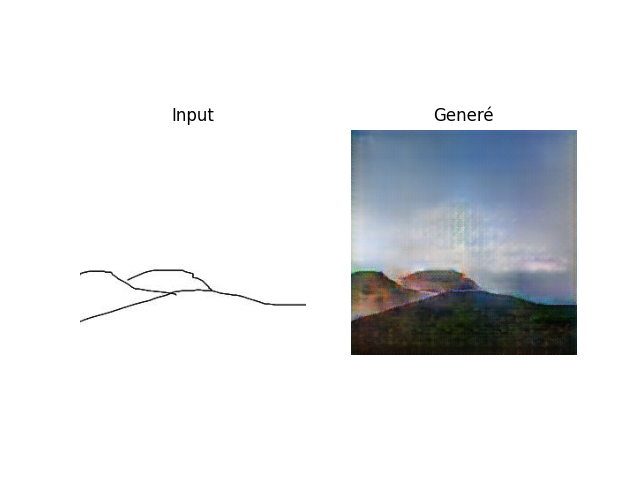
\includegraphics[width=0.7\linewidth]{images/pix2pix-t1.png}

Il est alors possible d'appliquer un transfert de style, dont l'image de contenu est la photo générée et l'image de style une peinture chinoise.

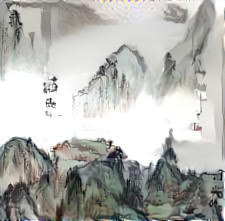
\includegraphics[width=0.7\linewidth]{images/pix2pix-t1-ts.jpg}

Au final il serait peut-être plus judicieux de fabriquer directement un dataset croquis/peinture chinoise, dont les peintures auraient été générées en appliquant un transfert de style à des photos.


\section{Problème des abstractions}

Nous l'avons vu il est possible de générer un paysage à partir de quelques lignes. Cependant, nous sommes confronté à un problème avec ce type de répresentation en entrée : 

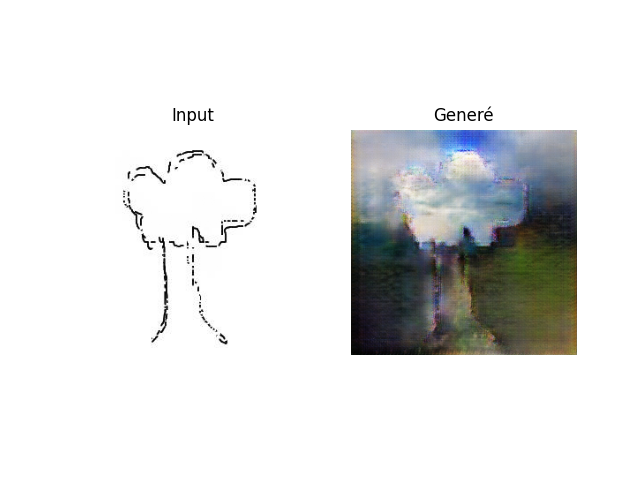
\includegraphics[width=0.7\linewidth]{images/pix2pix-fail.png}

En effet, le model n'as pas été confronté à ce type d'entrée, il n'est donc pas en mesure de faire le lien avec un arbre "réel". 

Voici les solutions envisagées  :
 
- Dessiner les croquis du dataset à la main. Théoriquement, cette solution pourrait fonctionner mais il existe deux inconvenients majeurs : c'est fastidieux, et puis il faut mobiliser le plus de participants différents afin d'avoir des abstractions variées. Enfin le dataset sera très proche de la problématique du "paysage chinois"

- Etre capable de générer une représentation abstraite à partir d'une photos ou d'une peinture. Nous pensons que le dataset quickdraw pourrait être un très bon point de départ.

Il existe cependant de gros problèmes, lié à l'orientation de l'objet (ref), et bien connu des hors champs.

- Enfin il y a également la piste des "sémantiques layouts", utilisées par GauGan. Nous ne pouvons pas considérer les sémantique layout comme des abstractions. Mais nous constatons qu'il est possible via ces dernier de résoudres efficacement le probleme.

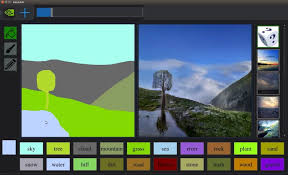
\includegraphics[width=0.5\linewidth]{images/gaugan-abs-ex.jpeg}

Il faudrait donc trouver le moyen de passer du croquis au sémantique layout


\chapter{Résultats et solutions apportées}


\chapter{Conclusion et Perspectives\label{chap-conclusion}}

\bibliographystyle{alpha}
\bibliography{memoire}
\end{document}
